%----------------------------------------------------------------------------------------
%	PACKAGES AND OTHER DOCUMENT CONFIGURATIONS
%----------------------------------------------------------------------------------------

\documentclass[final]{beamer}

\usepackage[framemethod=TikZ]{mdframed}
\usepackage[orientation=portrait, scale=1.24]{beamerposter} % Use the beamerposter package for laying out the poster
\usepackage[percent]{overpic}
\usepackage{amsmath}
\usepackage{amssymb}
\usepackage{gensymb}
\usepackage[T1]{fontenc}
\usepackage{color}
\usepackage{graphicx}  % Required for including images
\usepackage{booktabs} % Top and bottom rules for tables

\usetheme[]{confposter} % Use the confposter theme supplied with this template

\setbeamercolor{block title}{fg=ngreen,bg=white} % Colors of the block titles
\setbeamercolor{block body}{fg=black,bg=white} % Colors of the body of blocks
\setbeamercolor{block alerted title}{fg=white,bg=dblue!70} % Colors of the highlighted block titles
\setbeamercolor{block alerted body}{fg=black,bg=dblue!10} % Colors of the body of highlighted blocks

\usefonttheme{professionalfonts}
\setlength{\paperheight}{44in}
\newlength{\sepwid}
\setlength{\sepwid}{0.024\paperwidth} % Separation width (white space) between columns
\newlength{\onecolwide}
\setlength{\onecolwide}{0.31\paperwidth} % Width of one column
\newlength{\twocolwide}
\setlength{\twocolwide}{0.464\paperwidth} % Width of two columns
\newlength{\threecolwide}
\setlength{\threecolwide}{0.708\paperwidth} % Width of three columns

\newlength{\readoutimgheight}
\setlength{\readoutimgheight}{5in}
\newlength{\readoutimgwidth}
\setlength{\readoutimgwidth}{10.5in}

\setlength{\topmargin}{-0.5in} % Reduce the top margin size
%-----------------------------------------------------------


\newcommand{\checkedbox}{\textcolor{dgreen}{$\text{\rlap{$\checkmark$}}\square$}}
\newcommand{\checkbox}{$\square$}
%----------------------------------------------------------------------------------------
%	TITLE SECTION
%----------------------------------------------------------------------------------------

\title{Telescope to Test CMS Pixel Upgrade Detectors} % Poster title

\author{\textbf{Caleb Fangmeier} \\
  \textit{on behalf of the CMS Collaboration}} % Author(s)


\institute{Department of Physics \& Astronomy \\ \textit{University of Nebraska \-- Lincoln}} % Institution(s)

%----------------------------------------------------------------------------------------

\mdfsetup{skipabove=\topskip,skipbelow=\topskip}
\mdfdefinestyle{curvedtranslucent}{%
  outerlinewidth=0pt,innerlinewidth=0pt,
  outerlinecolor=gray,
  roundcorner=8pt,
  tikzsetting={fill=White,
               fill opacity=0.9},
  backgroundcolor=none
}
\mdfdefinestyle{simpleblack}{%
  outerlinewidth=2pt,innerlinewidth=0pt,
  outerlinecolor=black,
  backgroundcolor=white
}
\begin{document}

\addtobeamertemplate{block end}{}{\vspace*{2ex}} % White space under blocks
\addtobeamertemplate{block alerted end}{}{\vspace*{2ex}} % White space under highlighted (alert) blocks

\setlength{\belowcaptionskip}{2ex} % White space under figures
\setlength\belowdisplayshortskip{2ex} % White space under equations

\begin{frame}[t] % The whole poster is enclosed in one beamer frame
% \begin{columns}
  \small
  % \begin{column}{0.66\textwidth}
  The innermost layer of the CMS Detector at the LHC is the silicon pixel tracker. The current version of the detector has performed well and been critical to the physics program of CMS\@.  However, as the LHC produces higher instantaneous luminosities and higher center-of-mass energies, the detector must be upgraded to accommodate. The HL-LHC Upgrade of CMS will replace the entire silicon tracking system.  As part of this upgrade, a proposed new section of the pixel tracker will be added in the so-called ``very-forward'' ($\eta\sim4$)region of the detector.  This new section of the detector will have different pixel geometries than the current detector, and these new geometries must be accurately characterized.  Therefore, a telescope is being developed for the express purpose of characterizing these sensors so the pixel geometry can be optimized before settling on a final design to be placed in CMS\@.
The telescope operates by using eight layers of silicon-strip sensors, with the device-under-test placed with four on each side. A charged-particle beam is directed so it passes through both the strip sensors and the device-under-test. Measurements from the telescope are taken to reconstruct individual particle tracks.
% \end{column}
% \begin{column}{0.33\textwidth}
%   \begin{figure}
%     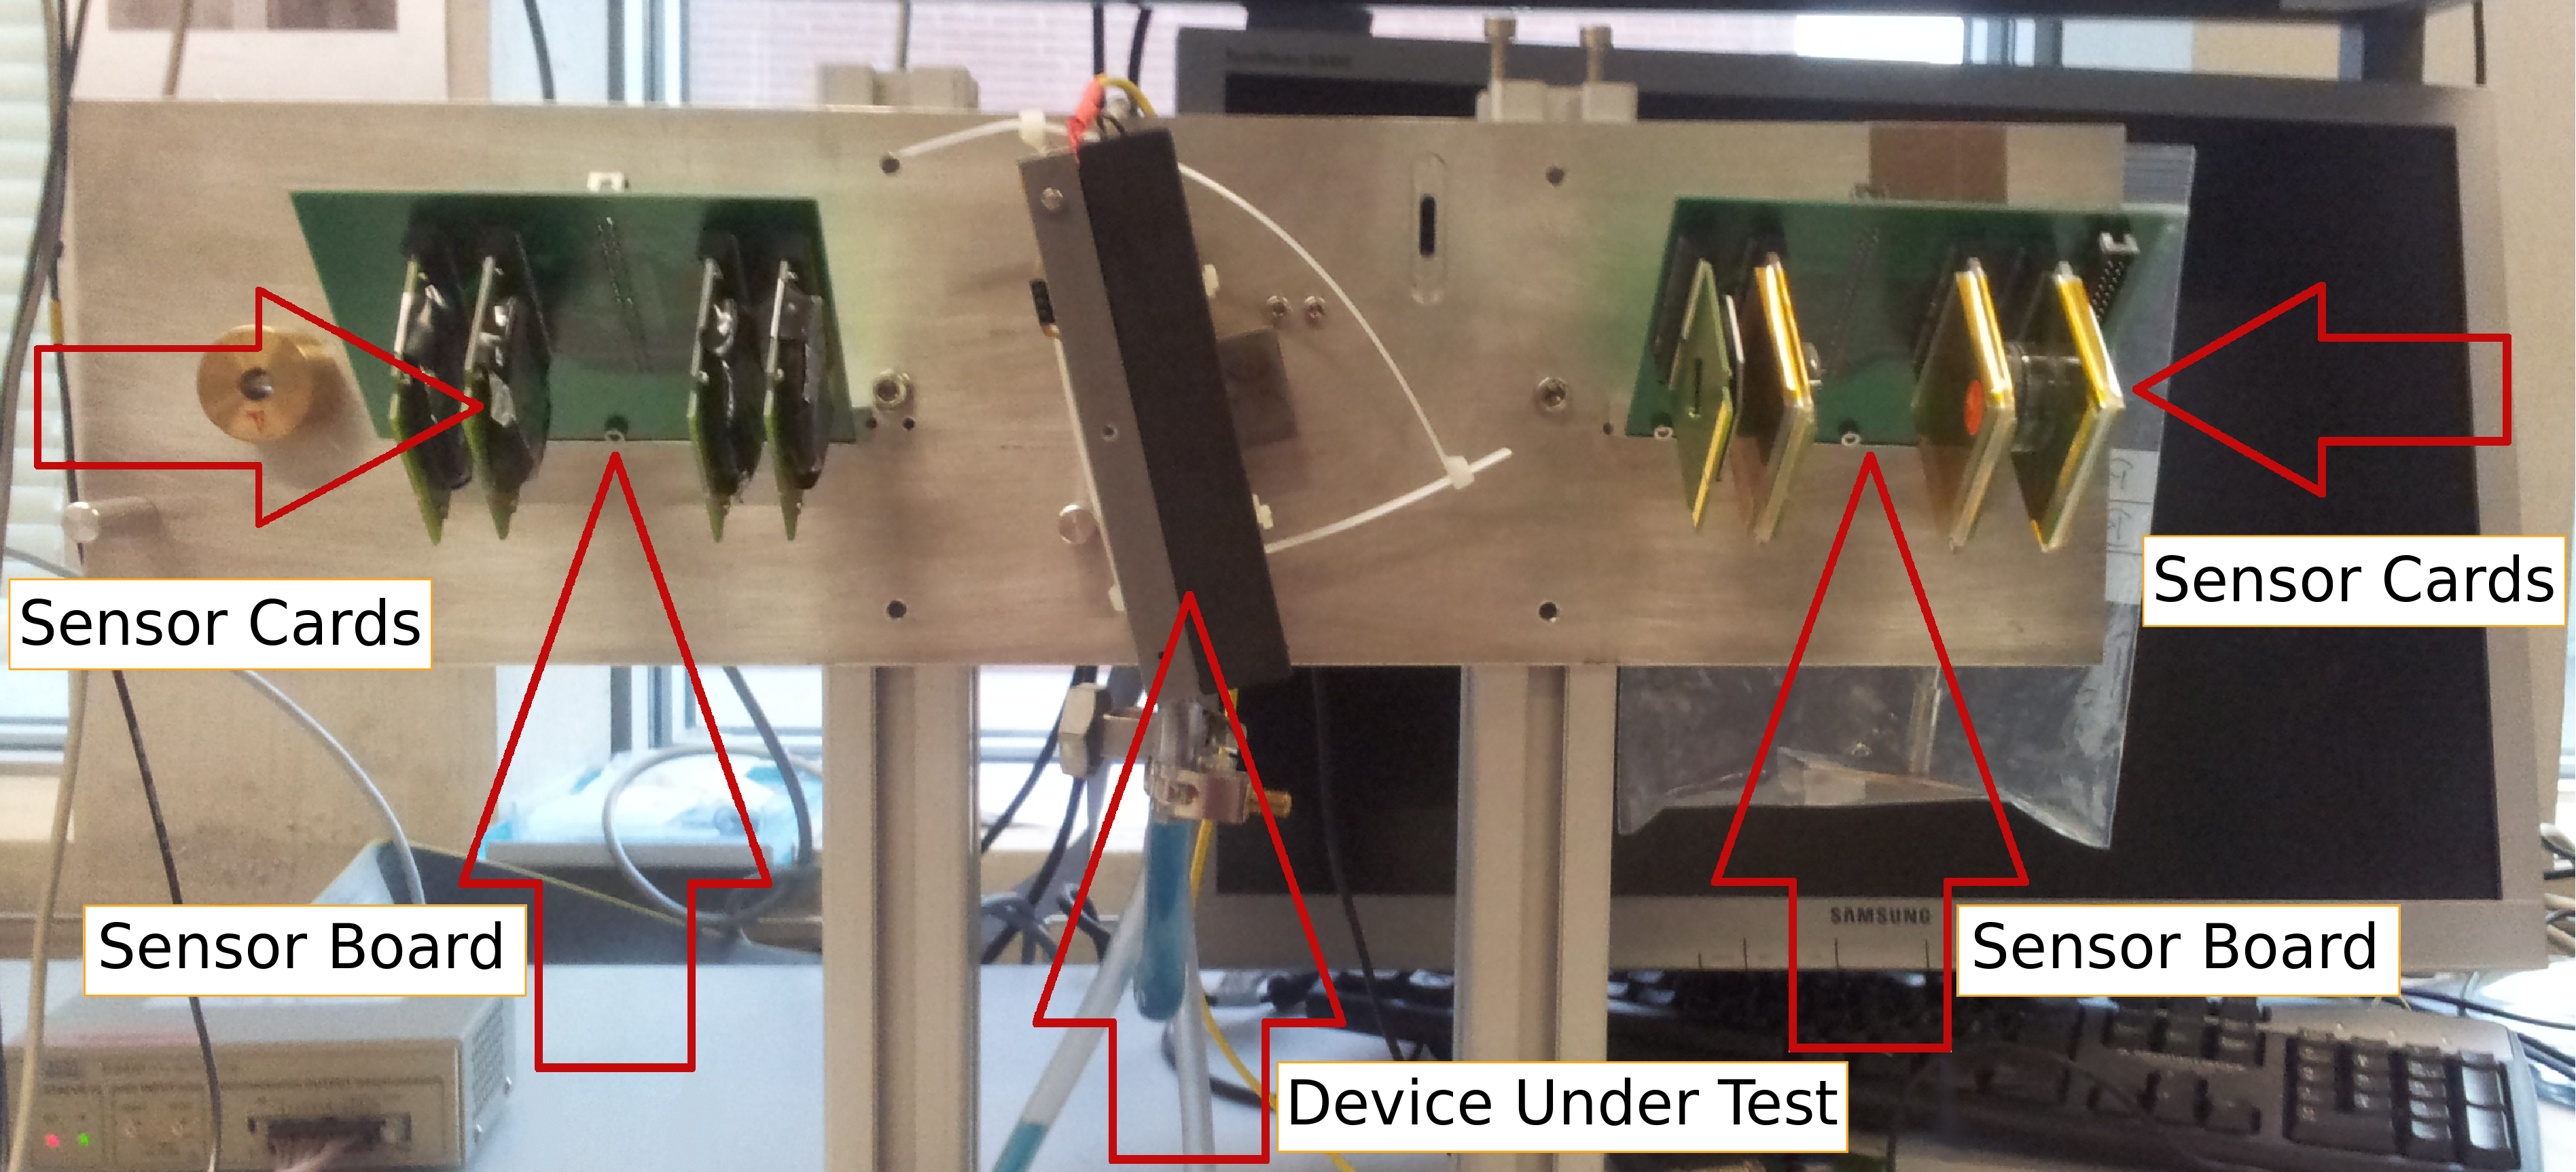
\includegraphics[width=\textwidth]{figures/Telescope_Old}
%   \end{figure}
% \end{column}
% \end{columns}
  
\vspace{.2in}

\begin{exampleblock}{Hardware}
  \begin{columns}[t]
    \begin{column}{\onecolwide}
      \begin{block}{Analog Pipeline Chip (APC-128)}
        \centering
        \begin{overpic}[height=5.5in, width=10in]{figures/APC128_Schematic}
          \put(4,7){%
            \begin{minipage}[t]{0.90\textwidth}
              \begin{mdframed}[style=curvedtranslucent]
                \footnotesize
                \begin{itemize}
                \itemsep0em 
                  \item Developed for the tracker of the H1 detector at HERA
                  \item Serializes the analog pulse-heights of 128 channels to dramatically reduce the number of required I/O lines
                  \item Capable of sampling waveform data from of a strip sensor at upwards of 20MHz
                  \item Features a very good signal-to-noise ratio of 40.
                  \item Low noise combined with inter-strip charge-sharing give each layer of the detector a measurement precision of $\approx\negthickspace1\mu$m
                \end{itemize}
              \end{mdframed}
            \end{minipage}
            }
        \end{overpic}
      \end{block}
    \end{column}
    \begin{column}{\onecolwide}
      \begin{block}{Sensor Board}
        \centering
        \vspace{-.1in}
        \begin{overpic}[height=5.5in, width=10in]{figures/Half-Telescope-Full}
          \put(4,7){%
            \begin{minipage}[t]{0.90\textwidth}
              \begin{mdframed}[style=curvedtranslucent]
                \vspace{.2in}
                \begin{columns}[t]
                  \begin{column}{.02\textwidth}\end{column} %Spacer column
                  \begin{column}{0.5\textwidth}
                    \textbf{Features}
                    \begin{itemize}
                      \itemsep0em 
                      \tiny
                      \item Each card can be used to measure either $x$ or $y$ track position
                      \item Configuration shown has alternating $x$ and $y$ measurements
                      \item Shared control signals for synchronous data taking
                      \item Individual output channels for fast readout
                      \item Fast readout is critical to minimize downtime
                    \end{itemize}
                  \end{column}
                  \vrule{}
                  \begin{column}{0.5\textwidth}
                    \textbf{Components}
                    \vspace{-.4in}
                    \begin{itemize}
                      \itemsep0em 
                      \tiny
                      \item 4$\times$ Sensor Cards, each with
                      \begin{itemize}
                        \itemsep0em 
                        \tiny
                        \item 1$\times$512-channel micro-strip sensor
                        \item 4$\times$APC-128
                        \item 4$\times$AD8138 buffer amplifiers
                        \item 4$\times V_{analog}$ trimmer potentiometers
                      \end{itemize}
                      \item 4$\times$RJ-45 Ports
                      \item 1$\times$40-Pin $.1$\textquotedbl~Header
                    \end{itemize}
                  \end{column}
                \end{columns}
              \end{mdframed}
            \end{minipage}
            }
        \end{overpic}
      \end{block}
    \end{column}
    \begin{column}{\onecolwide}
      \begin{block}{Data Acquisition (DAQ) Board}
        \centering
        % \begin{overpic}[height=5.5in, width=10in]{figures/DAQCard2015_Full_Front}
        \begin{overpic}[height=5.5in, width=10in]{figures/DAQ_Board_Real.png}
          \put(4,7){%
            \begin{minipage}[t]{0.90\textwidth}
              \begin{mdframed}[style=curvedtranslucent]
                \vspace{.2in}
                \begin{columns}[t]
                  \begin{column}{.02\textwidth}\end{column} %Spacer column
                  \begin{column}{0.50\textwidth}
                    \textbf{Features}
                    \tiny
                    \begin{itemize}
                      \itemsep0em 
                      \item Generates the control signals needed by the APC-128s
                      \item 32 ADC Channels to read out all APC128s in parallel, minimizing dead time
                      \item FPGA Board with associated USB hardware enables high-speed communication with online software.
                      \item Handles external triggering from a variety of sources via an translator mezzanine card.
                    \end{itemize}
                  \end{column}
                  \vrule{}
                  \begin{column}{0.50\textwidth}
                    \textbf{Components}
                    \vspace{-.4in}
                    \begin{itemize}
                      \itemsep0em 
                      \tiny
                      \item $1\times$\textbf{\textit{Opal Kelly} ZEM4310} with
                        \begin{itemize}
                          \itemsep0em 
                          \tiny
                          \item Cyclone IV FPGA
                          \item 128MB RAM
                          \item USB-3.0
                          \item $2\times$HSMC Connectors
                        \end{itemize}
                      \item $8\times$AD9219 40MHz/10 bit ADCs
                      \item $8\times$RJ-45 Ports
                      \item $2\times$40-Pin $.1$\textquotedbl~Header
                      \item Bias-voltage control relay
                      \item On-board power regulation
                    \end{itemize}
                  \end{column}
                \end{columns}
              \end{mdframed}
            \end{minipage}
            }
        \end{overpic}
      \end{block}
    \end{column}
  \end{columns}
\end{exampleblock}

\vspace{2.7in}
\begin{exampleblock}{Readout Scheme}
  \begin{columns}[t]
    \begin{column}{\onecolwide}
      \begin{figure}
        \centering
        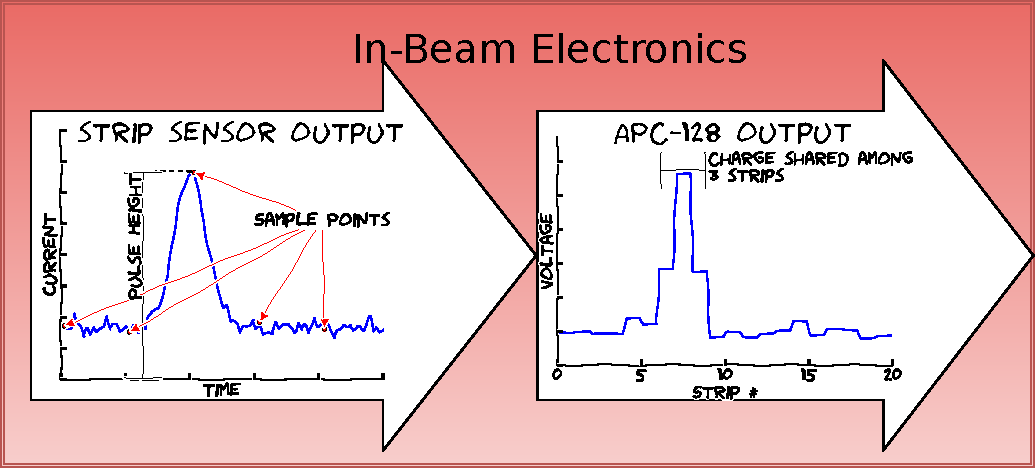
\includegraphics[height=\readoutimgheight, width=\readoutimgwidth]{figures/Telescope_Data_Flow_Stage_I.pdf}
      \end{figure}
        \begin{itemize}
        \footnotesize
        \itemsep0em 
          \item The sensor is a silicon NP-Junction operated in ``reverse-bias'' mode where all free charge carriers are evacuated
          \item An energetic charged particle passing through the silicon deposits energy to create free electron-hole pairs which are then separated by the electric field produced by the biasing voltage
          \item The electrons create a current spike that the readout chip, the APC-128, samples and stores
          \item Upon receiving a trigger, the APC-128 serializes the analog pulse-height sample from each of the 128 channels
        \end{itemize}
    \end{column}
    \begin{column}{\onecolwide}
      \begin{figure}
        \centering
        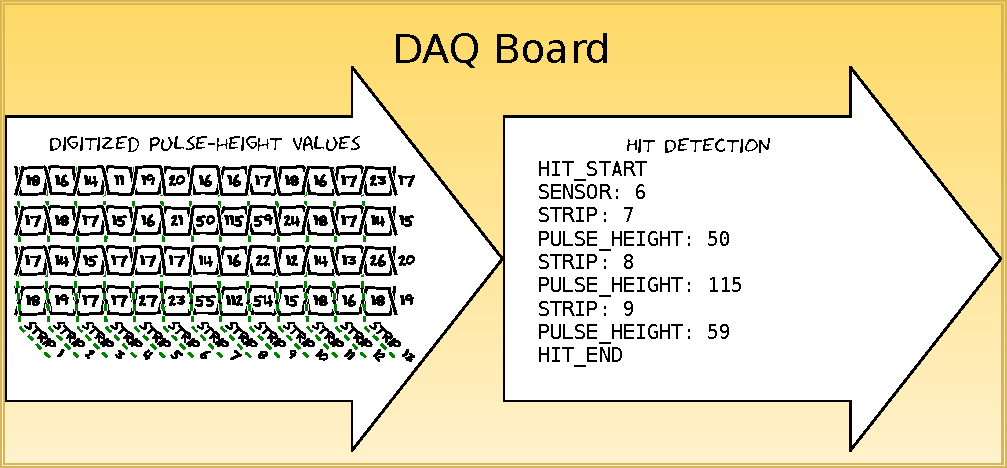
\includegraphics[height=\readoutimgheight, width=\readoutimgwidth]{figures/Telescope_Data_Flow_Stage_II.pdf}
      \end{figure}
      \footnotesize
      \begin{itemize}
      \itemsep0em 
        \item The analog pulse-heights from the 32 APC-128 in the telescope are digitized by 8 high-speed 4-channel ADCs located on the DAQ board
        \item The digitized values passed to an FPGA board where they are processed into individual sensor hits
        \item Digitized values smaller than the noise-suppression threshold are dropped
        \item The sensor hit data is passed across a USB-3 connection to a PC.\@
        \item Its job finished, the DAQ Board becomes idle and waits for the next trigger.
      \end{itemize}
    \end{column}
    \begin{column}{\onecolwide}
      \begin{figure}
        \centering
        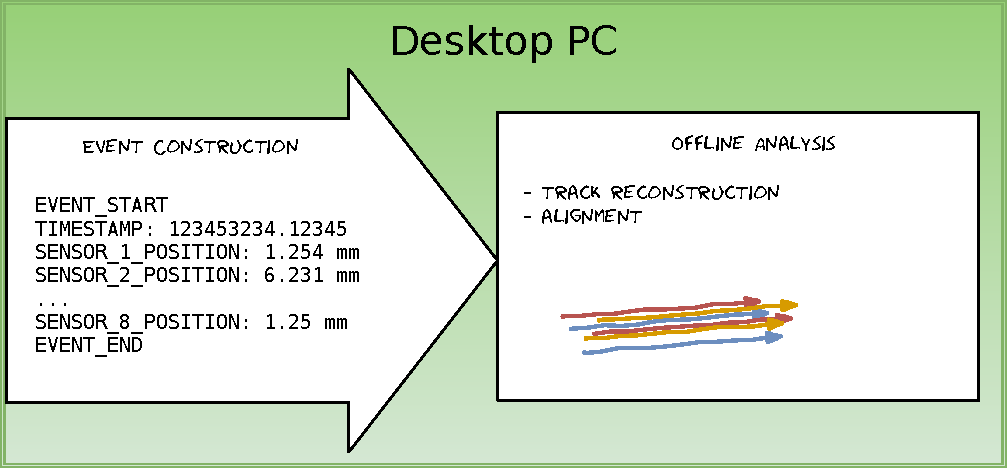
\includegraphics[height=\readoutimgheight, width=\readoutimgwidth]{figures/Telescope_Data_Flow_Stage_III.pdf}
      \end{figure}
      \footnotesize
      \begin{itemize}
        \itemsep0em 
        \item Online software organizes the hits into events and stores them to disk
        \item Since the detector layers can shift in space significantly during operation, alignment must first be done to accurately measure the geometry of the detector.
        \item After alignment, the various layer hits can be combined to construct extremely precise tracks.
        \item The tracks can then be compared for consistency with the data collected in parallel from the device-under-test, and, using the telescope as the ground truth, establish performance characteristics.
      \end{itemize}
    \end{column}
  \end{columns}
\end{exampleblock}


\begin{columns}[t]
  \begin{column}{\onecolwide}
    \begin{block}{APC-128 Testboard}
    \begin{overpic}[height=5.5in, width=10in]{figures/APC-128_Testboard.png}
      \put(4,10){%
        \begin{minipage}[t]{0.90\textwidth}
          \begin{mdframed}[style=curvedtranslucent]
            % \vspace{.2in}
            \footnotesize
            A custom board was developed for gaining familiarity with the APC-128 chip, and for testing different control and readout schemes. It features:
            \begin{itemize}
              \item $1\times$ APC-128 (bottom of board)
              \item 40-Pin header for supplying control signals
              \item $1\times$RJ-45 jack for testing differential output stage
              \item Automatic \emph{and} manual adjustment of analog reference voltages
            \end{itemize}
          \end{mdframed}
        \end{minipage}
        }
    \end{overpic}
    \end{block}
  \end{column}
  \begin{column}{\onecolwide}
    \begin{alertblock}{Progress}
      \checkedbox System design and parts selection \\
      \checkedbox APC-128 read out chain proof of concept\\
      \checkedbox Circuit design and PCB Layout \\
      \checkbox Assembly and offline testing (in progress)\\
      \checkbox FPGA Firmware development and testing \\
      \checkbox Online/Offline software development \\
      \checkbox Commissioning runs with UNL Diocles electron beam
    \end{alertblock}
    \vspace{.9in}
    \setbeamercolor{block alerted title}{fg=black,bg=norange} % Change the alert block title colors
    \setbeamercolor{block alerted body}{fg=black,bg=white} % Change the alert block body colors
    \begin{alertblock}{Contact Information}
      \begin{itemize}
      \item Email: \href{mailto:cfangmeier2@huskers.unl.edu}{cfangmeier2@huskers.unl.edu}
      \item Phone: +1 (402) 768 1358
      \end{itemize}
    \end{alertblock}
  \end{column}
  \begin{column}{\onecolwide}
    \begin{center}
      \begin{overpic}[height=0.7\onecolwide, angle=90]{figures/proposed_pixels}
        \put(4,5){%
          \begin{minipage}[t]{0.6\onecolwide}
            \begin{mdframed}[style=curvedtranslucent]
              % \vspace{.1in}
              \footnotesize
              Possible prototype pixel sensor layout to improve $p_T$ resolution in the forward region
            \end{mdframed}
          \end{minipage}
          }
      \end{overpic}
    \end{center}
    \vspace{.4in}
    \setbeamercolor{block title}{fg=red,bg=white} % Change the block title color
    \begin{block}{References} 
      \tiny
      \begin{itemize}
        \item ``Proposal for R&D Related to the Module and Sensor Design for the Phase-2 Upgrade of the CMS Forward Pixel Detector'' A. Dominguez et al. \textit{CMS Document 12163-v1}
        \item \textbf{PCB Design Files:} https://github.com/cfangmeier/VFPIX-telescope-PCB
        \item \textbf{Software Repository} https://github.com/cfangmeier/VFPIX-telescope-Code
      \end{itemize}
    \end{block}
    \setbeamercolor{block title}{fg=red,bg=white} % Change the block title color
    \begin{block}{Acknowledgments} 
      \footnotesize
      Beat Meier \& Tilman Rohe of \textbf{The Paul Scherrer Institute}\\
      Frank Meier of \textbf{Heidelberg University}\\
      Aaron Dominguez \& Rachel Bartek of \textbf{Catholic University of America}
      Brian Farleigh \& Bob Kelty of \textbf{University of Nebraska \-- Lincoln}
    \end{block}
  \end{column}
\end{columns}

\end{frame} % End of the enclosing frame

\end{document}

